\section{ICD in Clusters}
\label{sec:clusters}

\subsection{NeAr Clusters}
We earlier studied how ICD can be utilized to determine the structure of
heteroatomic rare gas clusters \cite{Fasshauer14_1} and thereby showed a clear
geometry dependence of the ICD electron spectra. Using the simulations of
cluster model structures, we were able to explain the shoulders of both
the NeNe-ICD and the NeAr-ICD peak by decay with decay partners of the next
shell. While the shoulder of the NeAr-ICD peak might be able to be explained
by a decay of higher vibrational levels \cite{Scheit06}. However, in neon
clusters no bound vibrational states exist \cite{}.
Other decay processes resulting in secondary electrons of the corresponding
kinetic energies between \unit[2.5]{eV} and \unit[3.5]{eV} are not known.
Therefore, we can conclude that this shoulder stems from next shell ICD.
In the following, we will zoom into the NeNe-ICD part of the spectra
of Figure xyz of Ref. \cite{Fasshauer14_1} and analyze them in more detail.

\label{sec:near}
\begin{figure}[h]
 \centering
 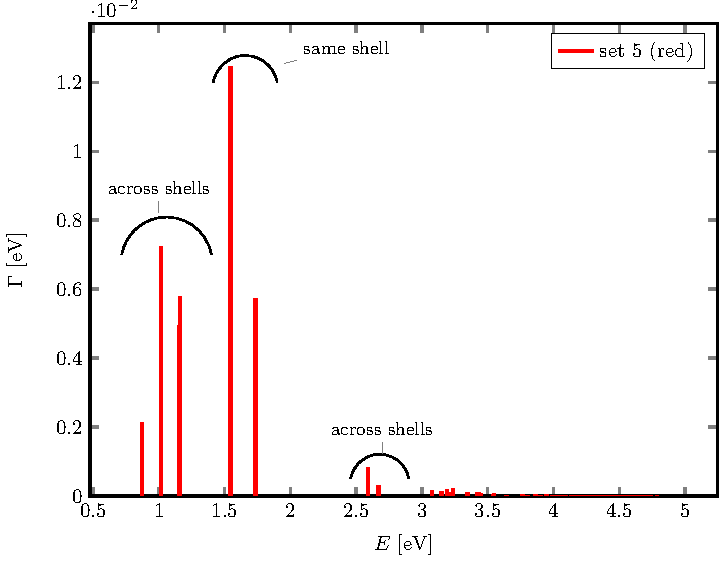
\includegraphics[width=\columnwidth]{pics/rot.pdf}\\
 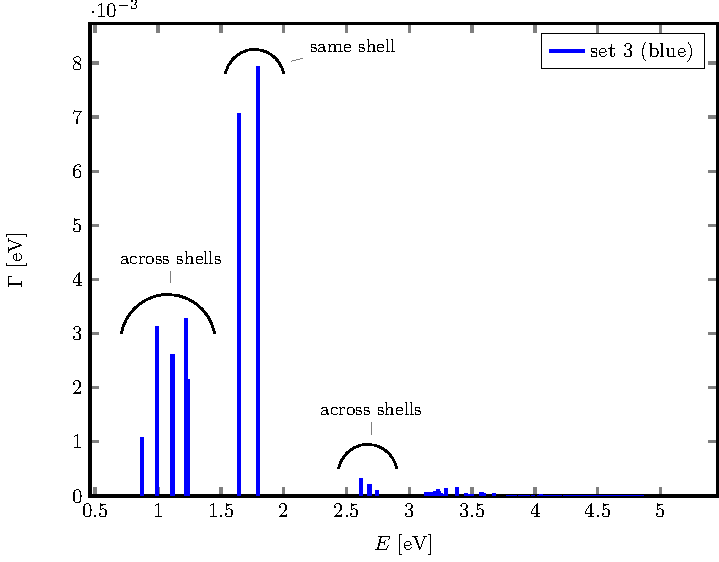
\includegraphics[width=\columnwidth]{pics/blue.pdf}
 \caption{ICD spectra for the NeNe-ICD part of the structures of set 3 and
          set 5 of the NeAr clusters in Ref. \cite{Fasshauer14_1}
          plotted as stick spectra.
          The different peak groups resemble different pair types
          within the NeAr clusters. The lowest energy peaks (\textbf{a})
          refer to nearest neighbours
          of different shells, the peak group \textbf{b} refers
          to nearest neighbours within one shell and the peak group \textbf{c}
          refers to next nearest neighbours between different shells.
          The peaks in group \textbf{d} contain both peaks stemming from
          pairs within the same shell as well as pairs consisting of atoms
          of different shells.}
 \label{figure:rot_blue}
\end{figure}

In Figure \ref{figure:rot_blue} the ICD electron spectra for the NeNe-ICD
part of heterogeneous clusters are shown as stick spectra
for set 3 and set 5. Hereby, we stick to the color code of
Ref. \cite{Fasshauer14_1}. Both spectra exhibit a similar pattern of peak groups.
The groups are found around \unit[1.0]{eV} (group \textbf{a}),
around \unit[1.7]{eV} (group \textbf{b}), around \unit[2.6]{eV} (group \textbf{c})
and from \unit[3]{eV} to \unit[4]{eV} (group \textbf{d}). By comparing
the interatomic distances, of which these peaks originate to their occurance
in the cluster structures, the peak groups can be assigned to atom pairs
within the cluster. For group \textbf{a} the peaks stem from decays
between two nearest neighbour atoms of two different shells, while group \textbf{b}
stems from the decay partners being nearest neighbours in the same shell.
Group \textbf{c} can be assigned to next-nearest neighbours in adjacent shells
and group \textbf{d} stems from a mixture of pairs which cannot unambigiously
be categorized because different kinds of peaks intersect each other.

Obviously, the peak groups have a fine structure which originates from
different positions of the decay partners within a shell (face, egde or vertex).
For the investigated ideal icosahedral structures, these pairs of group \textbf{a}
are from low to high kinetic energies: vertex-vertex, edge-edge, edge-face and
face-face. Due to vibrational broadening of the peaks the experimental observation
of this fine structure is unlikely in neon clusters.

Concluding these findings, there is not neccessarily only one kind of nearest
neighbours in clusters. Even the next-nearest neighbours are closer to
twice the interatomic distance of the closest pair with an open decay channel.
Therefore, as formerly supposed, decay partners of twice the closest interatomic
distance indeed have a very small contribution to the total spectrum. However,
all other decay partners do have to be taken into account in order to simulate
an ICD spectrum for clusters.


\subsection{Icosahedral vs. Cuboctahedral Structure of Clusters}
\label{sec:icofcc}
We would like to recall that clusters with an icosahedral structure
have shorter interatomic distances between shells then within the same
shell.
In terms of the ICD, different groups of nearest neighbours exist,
one within the same shell and one
between adjacent shells. This is characteristic for icosahedral cluster structures.
Cuboctahedral cluster structures on the other hand are characterized by only
one interatomic distance. 
Therefore, icosahedral cluster structures should be distinguishable from
cuboctahedral clusters by the number of peaks as shown in Figure
\ref{figure:reinNe}.

\begin{figure}[h]
 \centering
 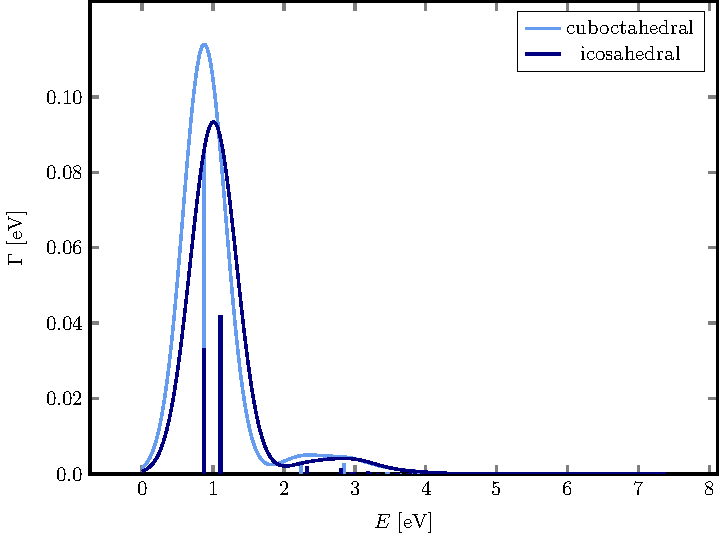
\includegraphics[width=\columnwidth]{pics/reinNe}
 \caption{ICD spectra of pure neon clusters consisting of 55 atoms in
          icosahedral and fcc structure. In clusters with an ideal fcc structure
          all interatomic distances are the same and hence only one peak
          for each shell around any atom in the cluster is to be expected.
          In ideal icosahedral clusters the interatomic distances between atoms
          within the same shell and between atoms in neighbouring atoms
          are different. Therefore two peaks for interactions partners
          at different distances can be expected. This feature might
          help to experimentally identify the underlying structure of clusters.}
 \label{figure:reinNe}
\end{figure}

Whether or not the cluster structures would be distinguishable in experiment
will depend the vibrational broadening of the peaks, the experimental
resolution and the distance difference and hence the energy difference of the
peaks in the icosahedral structure. In this proof-of-principle discussion
we chose neon clusters for comparison with experiment but for the distinction
of cluster structures it might be recommendable to choose atoms with larger
internuclear distances in clusters.

